\documentclass[a4]{article}
%\usepackage{czech}
\usepackage{graphicx}
\usepackage[utf8]{inputenc}   % pro unicode UTF-8
\usepackage{booktabs}
\usepackage{hyperref}
%#\usepackage{qtree}
%\usepackage{graphviz}
\usepackage{authblk}
%\usepackage{tikz-dependency}
\usepackage[ampersand]{easylist}

\usepackage{verse}

\def\furl#1{\footnote{\url{#1}}}


\begin{document}

\title{Automatic accentual-syllabic poet}

\author{Dominik Macháček}
\affil{
Saarland University, Saarbrücken, Germany,
dominik.machacek@matfyz.cz
}

\date{\today}

%\pacs{PACS numbers go here. These are classification codes for your  research. See {\tt http://publish.aps.org/PACS/} for more info.}
\maketitle

%\begin{abstract}
%TODO: An abstract is a great convenience for the reader and is required by all journals.
%\end{abstract}


\section{Introduction}

Our task is to create a generator of an accentual-syllabic poetry.

Verses in this kind of poetry are restricted by the rhythm of accents, all
verses must have given number of syllables and the verses in a strophe
rhyme by the chosen pattern. See example in figure \ref{may}.

\def\surl#1{%
    {\footnotesize\url{#1}}%
}%

\begin{figure}[ht]
\label{may}
\centerline{
I {\bf know} a {\bf glade}, spring {\bf crys}tal {\bf clear},
}
\centerline{
in {\bf dee}pest {\bf wood}land, {\bf crowned}
}
\centerline{
by {\bf sha}dy {\bf ferns} in {\bf si}lhou{\bf ettes},
}
\centerline{
red {\bf hea}ther {\bf all} a{\bf round}.\footnotemark
}
\caption{Bold syllables are stressed, other syllables are non-stressed.
There is a regular pattern of stressed and non-stressed
syllables in each verse. Second and fourth verse rhyme.
}
\end{figure}


\footnotetext{From "The Crystal Spring" by J. V. Sládek, translated by
Václav Z J Pinkava.
Available at \url{http://www.vzjp.cz/basne.htm\#Sladek}.
}


% Summary?


In this project we make an automatic generator of accentual-syllabic
poems. Its input are a poetic form, namely a pattern of stressed and
non-stressed syllables in each verse, and a raw coherent Czech text. The
whole process of generating is fully automatic, no manuall anotation of
the text is needed.

On the output there are poems compounded from newly-created nonsense words
reminding Czech language. They are pronouncable and they precisely
fit into the given poetic form.

\section{Motivation}

Accentual-syllabic poetry is very popular genre in many national cultures
including Czech, English and German. Poems written by human
poets are usually written in some variety of natural language, their words
have meaning and the whole poem has some intention.
To write a good poem is a difficult task, a poet must choose proper words
and fit them into a pleasant form. 

We want to make an automatic poems generator because with it new poems can
be easily created by computer. They will be unique, interesting and
entertaining pieces of art. They could also be published for general public
and draw attention to the whole field of Computational Linguistics.

\section{Related works}

We can find works from other authors more or less related to our topic, but
there isn't any work providing accentual-syllabic poetry generator for Czech. 
Related works are described in this section.

\subsection{Poem generators with restricted originality}

On the Internet we can find several
sites called "poems generators", which are in fact simple games producing texts with
very restricted originality. They ask a user for a set of input words and then
they put them into a static template. Results usually don't have a fixed rhythm
and they usually don't rhyme. See table \ref{tab:gen} for example of such generators.

\begin{table}[ht]
\begin{tabular}{ll}
\hline
{\bf name} & {\bf URL} \\
\hline
\hline
AI poem & \surl{http://www.aipoem.com/easypoem/} \\
Poem Generator & \surl{http://thinkzone.wlonk.com/PoemGen/PoemGen.htm} \\
PoemOfQuotes & \surl{http://www.poemofquotes.com/tools/poetry-generator.php} \\
\hline
\hline
\end{tabular}
\caption{}
\label{tab:gen}
\end{table}


\subsection{Short poems of restricted form}

There are restricted poem forms having small length and a simple constraints
verifiable by computer.
Computer programs can be used to generate or to seek them in a big corpus.
For example snowballs are sentences where every word is one letter longer
than the previous. A computer can find such words in a corpus and put them
together to create a meaningful sentence. 
Summary\footnote{We have taken most of them from following source:
\url{http://mentalfloss.com/article/57715/14-hilarious-automatic-text-and-tweet-generators-flair-poetry-and-language-play}  
}
of such works is in table \ref{tab:rest}.

\begin{table}[ht]
\begin{tabular}{lll}
\hline
{\bf name} & {\bf URL} & {\bf form} \\
\hline
\hline
Snowball poetry & \surl{https://twitter.com/snowballpoetry}
& snowball \\
Pentametron & \surl{https://twitter.com/pentametron} & iambic pentameter \\
Anagramatron & \surl{https://twitter.com/anagramatron} & anagrams \\
HAIKU9000 & \surl{https://twitter.com/HAIKU9000} & haiku \\
Pangramtweets & \surl{https://twitter.com/PangramTweets} & pangrams \\
\hline
\hline
\end{tabular}
\caption{}
\label{tab:rest}
\end{table}

\subsection{Neural network poetry}

In other group of works state-of-the-art deep learning techniques are used
to generate poetry. They put effort to make a poem with a deep meaning, but
use a loose form of a free verse. Some of them also aim to artificially
create poems which would pass Turing test, it means to be judged by humans
as created by humans and not by bot. They can be found on the site "Bot or
not"\furl{http://botpoet.com/}.

Some of the works related with neural network poetry can be found in
table \ref{tab:nn}.

\begin{table}[ht]
\begin{tabular}{lll}
\hline
{\bf name} & {\bf URL} \\
\hline
\hline
A Neural Network's Poetry  & \surl{http://neuralnetpoetry.blogspot.de/} \\
NeuralSnap & \surl{https://github.com/rossgoodwin/neuralsnap} \\
\hline
\hline
\end{tabular}
\caption{}
\label{tab:nn}
\end{table}

% Slovak generator of Vogon poetry: http://www.ludoslovensky.sk/slova/vogon/
% could be also somehow mentioned


\subsection{Poetweet}

There exists a site poetweet\furl{http://poetweet.com.br/}, where a user
fills a Twitter channel and then chooses a poem type. He can choose either a sonnet,
rondel or indriso, that are a fixed forms of accentual-syllabic poetry.
Afterwards, tweets from the Twitter channel are extracted and a poem is
created from tweets' coherent excerpts. It also provides links for
mentioned tweets.

Poetweet doesn't have any restrictions on the channel's language and
doesn't provide any information about its inner design. It could be
intended for Portuegese and could use language-specific processes. Also the
poem form and source domain are very restricted.

Poems from Czech Twitter channels doesn't have a strict good-quality rhythm,
but they have rhymes.
%Poetweet also shows that using coherent text excerpts
%is a good idea, .


\section{Solution}

Generator's workflow consists of two phases, training and generating. 

In
training phase, an input text is preprocessed and splitted to syllables.
Then stresses are indicated.  Finally, a language model is created from list
of syllables and their accents.

In generating phase, a language model is used for creating of a poem by given form.

More detailed descriptions of each mentioned process follow in special subsections.

Our generator can work for arbitrary natural language, but we work with
Czech. Reasons for this decision is that there exist many
resources of Czech texts, we can use an automatic tool for splitting text to syllables,
and the word-stress in Czech language is very regular so we can indicate
it automatically. Czech is also a native language of the author of this
project, so we are able to evaluate the quality of resulting poems. 

For some other languages we should use either a special tools for splitting
to syllables and for accent indication (which we don't have for any other
language including English),
or we could use a corpus annotated with syllables and accents, but this
restricts the domain and size of input texts.


\subsection{Text preprocessing}

In text preprocessing we do tokenization and sentence segmentation, because
following syllabification and accentification steps require single sentences. We also
remove punctuation and digits and transform text to lowercase. This decreases number of
unique syllables and makes language model more inovative, although it losts
some information.

For tokenization and segmentation we use NLTK Punkt tokenizer \cite{nltk}. % reference

\subsection{Syllabification}

For automatic syllabification we used Sekáček\cite{sekacek}.
It's a Python implementation of static rules created by experts on this
issue. The algorithm was described by Jitka Štindlová\cite{naserec}.
It's intended only for Czech.

\subsection{Accents}

Resource as\cite{prizvuk} state that Czech is a language with
a fixed accent. It's always on the first syllable of a word with only some exceptions: 

-- monosylabic prepositions are so called enclitics, they take accent from
following word and therefore they're accented. 

%Example without
%prepostition: {\bf o}ke{\sl nní} {\bf
%rám}, with prepostion {\bf pod} o{\sl ke}nním {\bf rá}mem (a window frame, under a window
%frame)

-- some function words as monosylabic (short forms of) personal and
reflexive pronouns or past tense and conditional's auxiliaries are clitics,
they always follow some word and are not accented %Example: 

-- in Czech poetry, a secondary accent is sometimes used, it's on the third and
fifth and every following odd syllable of a word

-- according to Rýmy.cz\cite{rymy}, monosyllabic words in poetry can be
sometimes read as accented and sometimes as non-accented, it depends on
it's position between other words

For our application we decided to implement only this rules. They hold in
majority of situations, but not always. For example, Jiří Zeman\cite{zeman} claims that
there are also articulatory influences leading to unstressed
pronunciation of monosylabic prepositions {\sl u, o} (near, about), if
following word starts with a vowel. %Compound words have also a secondary stress on
%a first syllable of second word, even if it

\subsubsection{Implementation}

We implemented a finite state transducer\cite{jurafsky} to mark every syllable as either 

-- primary stressed

-- unstressed

-- secondary stressed -- it's every third or following odd syllable in
a word and also monosylabic word apart from clitics

In a stress pattern, secondary stressed syllables can hold as either
stressed or unstressed.  
For clitics detection we created a static list.


\subsection{Language model}

We used N-gram language model. One unit of model is
a syllable, its accent (we destinguish primary, secondary and unstressed)
and its position in a word, it can be either initial, middle, trailing or
initial and trailing at once (for monosylabic words). For example, a word
"papa" consists of two different syllables, one is "pa-" and the other is
"-pa".

For every (N-1)-gram of syllables/accents pair, probabilities of next
syllables by given accents are estimated by maximum likelihood estimation
from the whole corpus. We don't use any smoothing. 

For generation of an initial N-gram we also compute the probabilities of
syllables by given N-grams of accents.

%Since a secondary stressed syllables can stand on a place of either primary
%stressed or unstressed syllables, we merge probabilities for generating of
%primary or secondary  syllables and for generating of unstressed or
%secondary.

Trivial example of unigram model is in table \ref{tab:model}.

\begin{table}[ht]
\centerline{
	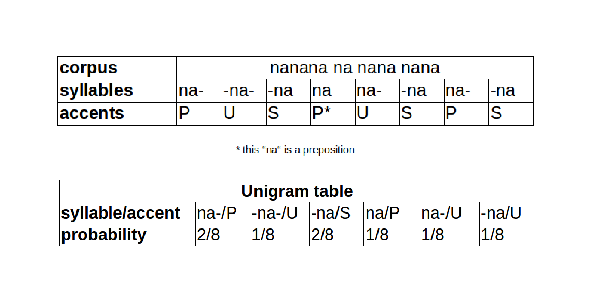
\includegraphics{corpus.pdf}
}
\caption{Example model.
}
\label{tab:model}
\end{table}




\subsection{Generating}

Generator has on its input a language model and a verse pattern, it's a sequence of symbols
denoting stressed or unstressed syllable. For generation of initial N-gram
by given stress, we select one N-gram matching the stress pattern. Then we
take last generated (N-1)-gram and randomly select the next syllable with given
stress by precomputed probability distribution, which is stored in a model.
We repeat this for the whole verse pattern.

If we can't continue because the last generated (N-1)-gram doesn't provide any
following syllable matching given stress, then we generate a new N-gram as
in the beginning and continue.

\subsubsection{Rhymes}


Rýmy.cz\cite{rymy} describes good-quality criteria of rhymes. Rhyme
shouldn't be trivial, for example a rhyme of two words of the same
grammatical category in the same grammatical form is considered as banal
and bad-quality.

Two words rhyme if the phonetical forms of their endings are similar. 
Therefore for a good rhyming we need a morphological tagging and
also a phonological transcription, because for example words "dětský" and
"pecky" rhymes, although their ortographical forms of their endings are not
the same. In our application, words have no meanings and
therefore no grammatical category.

We decided to avoid the issue with a rhyme by simple way:
If two verses should rhyme, then we simply replace the last syllable of the
second verse with the last syllable of the first verse.

\section{Example outputs}

We tried to generate poems from different types of texts, from novels,
scientific paper, Facebook page and also from longer accentual-syllabic
poems and poem collection. We also experimented with different values of
N for N-gram model. This experiments are commented and reported here: 
\url{https://github.com/Gldkslfmsd/automatic-poet/blob/master/results.txt}.

Our observations show that the poems mostly have the intended rhythm. This
rhythm is more regular and has better quality, if we use poems on the
input. 

On this place we're including some of the generated poems. The poems
in italics are attempts for English translations of previous ones.


%\newcommand{\attrib}[1]{%
%\nopagebreak{\raggedleft\footnotesize #1\par}}
%\renewcommand{\poemtitlefont}{\normalfont\large\itshape\centering}


%\poemtitle{Mathematics}
\settowidth{\versewidth}{Than Tycho Brahe, or Erra Pater:}
\begin{verse}[\versewidth]
temný  letí  pomstu  dvory \\
bludinu  svou  v matku  mém  dvě \\
v bledé  tváře  bledou  barví \\
v lebku  slavík  růžila  zář  \\
\end{verse}

\settowidth{\versewidth}{Than Tycho Brahe, or Erra Pater:}
\begin{verse}[\versewidth]
%literal translation: \\
\it
dark he flies revenge dooryards \\
his strayeress, mother my two\\
in her pale face he dyes her pale\\
nightingale to skull, radiance rosed\\
\end{verse}
%\attrib{Samuel Butler (1612--1680)}

\settowidth{\versewidth}{Than Tycho Brahe, or Erra Pater:}
\begin{verse}[\versewidth]
k vůve jedži  deha  hletě \\
zaba  po jím  oné půj díš \\
a vo druní  zvon  a  hluku \\
krola  zde bě  já cha klobu\\
\end{verse}

\settowidth{\versewidth}{Than Tycho Brahe, or Erra Pater:}
\begin{verse}[\versewidth]
zamratě  nala  vždyc se  rá\\
kamena  tu  přežáry  a \\
libuše  i  nyní  trouby \\
všecko  mého  vraného  a \\
\end{verse}

\settowidth{\versewidth}{Than Tycho Brahe, or Erra Pater:}
\begin{verse}[\versewidth]
\it
she na-ed zamratessly her allw rah\\
she stoned -- here over-heats and\\
Libushe also now ovens\\
everything with my black and\\
\end{verse}

\settowidth{\versewidth}{Than Tycho Brahe, or Erra Pater:}
\begin{verse}[\versewidth]
život  s věčnou  smrtí  sbratřil \\
ženu  vábí  málo  zlato \\
jeho  kosti  a  hle  stříbro \\
klečí  klečí  nad  vodou  jsem\\
\end{verse}

\settowidth{\versewidth}{Than Tycho Brahe, or Erra Pater:}
\begin{verse}[\versewidth]
\it
life brothered with eternal death -- \\
woman's attracted by gold a little -- \\
his bones -- and look -- silver\\
he kneels, he kneels -- above the water I am!\\
\end{verse}


\settowidth{\versewidth}{Than Tycho Brahe, or Erra Pater:}
\begin{verse}[\versewidth]
pro  vši  víru  dobrých  lidí \\
tělo  mrtvo  leží  ani \\
komu  káže  slovo  lidské \\
ježí  celou  tíží  na  ní \\
\end{verse}

\settowidth{\versewidth}{Than Tycho Brahe, or Erra Pater:}
\begin{verse}[\versewidth]
\it
For all faith of good people\\
a death corpse lies neither.\\
To whom a human word preaches,\\
she bristles on her with all her weight.\\
\end{verse}






\settowidth{\versewidth}{Than Tycho Brahe, or Erra Pater:}
\begin{verse}[\versewidth]
smysl  věty  v jeho  pracích \\
kuda  chočet  jechať  chazcích \\
názvu  sprechtakt  jehož  užil \\
skládá  z jedné  nebo  z něžil\\
\end{verse}

\settowidth{\versewidth}{Than Tycho Brahe, or Erra Pater:}
\begin{verse}[\versewidth]
větší  váhu  nežli  ostat\\
touto  větší  vahou  tímstat\\
i  don  t  know  who  put  the  i \\
přízvuk  slovní  nýbrž  pří i \\
\end{verse}



\settowidth{\versewidth}{Than Tycho Brahe, or Erra Pater:}
\begin{verse}[\versewidth]
cídým  prečá zabo  pudek \\
odpiš ten tonénor zoká\\
zmužli renčej chceda z ka to \\
šlo po zmužjlep se ži daci\\
\end{verse}


\settowidth{\versewidth}{Than Tycho Brahe, or Erra Pater:}
\begin{verse}[\versewidth]
líbí  odpoťa  myří  ov\\
ovčáček  jak  školní  pan  hans \\
směrem  k modesádě  jsou  hnůj \\
obvykle  na  svou  ničemu \\
\end{verse}

\settowidth{\versewidth}{Than Tycho Brahe, or Erra Pater:}
\begin{verse}[\versewidth]
\it
Like it restier moush ov\\
shepherdy how school Mr. Hans\\
direction to modesade are mist\\
usually to his to nothing\\
\end{verse}

\settowidth{\versewidth}{Than Tycho Brahe, or Erra Pater:}
\begin{verse}[\versewidth]
zmizik  lukas  zmizik  vondra \\
střelba  pana  prezidenta \\
v lukáš  musil  lukáš  musil \\
leden  v lukas  zmizik  lukas \\
\end{verse}

\settowidth{\versewidth}{Than Tycho Brahe, or Erra Pater:}
\begin{verse}[\versewidth]
\it
Eraser Lucas Eraser Clement\\
a shooting of Mister President\\
Lucas Had-to Lucas Had-to\\
January Lucas Eraser Lucas\\
\end{verse}





\section{Conclusion}

We used an N-gram language model for syllables for generating accentual
poems from Czech syllables. Quality and originality of the poems depend on the input text
domain and the parameter N, but we can say that we are able to generate
interesting poems with regular rhythm.

\subsection{Future work}

Our work can be expanded by several ways. We can implement backtracking
algorithm to seek rhytmical patterns of given length in a coherent text or in the N-gram
model. We can add another restrictions so a verse can be a full grammatical
sentence, or at least the verse will begin and end with actual word
boundaries. Another restriction can be also to find rhyming verses.
We can also implement metrics for the quality of a verse and
find verses with at least acceptable quality. 

\pagebreak


\begin{thebibliography}{99}

\bibitem{nltk}
 {\sl NLTK: Nature Language Toolkit}

\bibitem{sekacek}
 {\sl Sekáček -- split Czech text to syllables}.
 \url{https://github.com/Gldkslfmsd/sekacek}


\bibitem{naserec}
 {\sl Jitka Štindlová: Dělení slov v češtině pomocí strojů}
(Word-splitting in Czech by machines). [1968] Published in {\sl Naše řeč}
(Our language),
{\sl year 51, number 1, pg. 23-32}. Available at
\url{http://nase-rec.ujc.cas.cz/archiv.php?art=5348}.


% TODO!!!
\bibitem{prizvuk}
 {\sl Marta Šimečková: Jak je to se slovním přízvukem v~češtině.} (How is
 it with a word-accent in Czech)
 \url{http://www.vaseliteratura.cz/teorie-literatury/144-slovni-prizvuk}


\bibitem{rymy}
 {\sl Pavel Šrubař: www.rymy.cz} (Rhymes.cz)
 \url{http://www.rymy.cz/rymy.htm}




\bibitem{zeman}
 {\sl Jiří Zeman: Ještě k přízvukování prvotních jednoslabičných
 předložek}
(Once again about a stress of monosylabic prepositions). [1983] Published in {\sl Naše řeč}
(Our language),
{\sl year 66, number 4, pg. 192-197}. Available at
\url{http://nase-rec.ujc.cas.cz/archiv.php?art=6402}.



\bibitem{jurafsky}
 {\sl  Dan Jurafsky and James H. Martin:	
 Speech and Language Processing
 }




\end{thebibliography}



%%%%%%%%%%%%%%%%%%%%%%%%%%%%%%%%%%%%%%%%%%%%



\end{document}

























%\centerline{
%Late {\bf eve}ning, {\bf on} the {\bf first} of {\bf May}—
%}
%
%\centerline{
%{\bf The} twilit {\bf May}—the {\bf time} of {\bf love}.
%}
%\centerline{
%{\bf Mel}tingly {\bf called} the {\bf turt}le-{\bf dove},
%}
%\centerline{
%Where {\bf rich} and {\bf sweet} {\bf pi{\bf ne}woods {\bf lay}.
%}
